% Chapter Template

\chapter{Feature Extraction} % Main chapter title
\label{Feature Extraction} % Change X to a consecutive number; for referencing this chapter elsewhere, use \ref{ChapterX}
\lhead{Chapter 4. \emph{Feature Extraction}} % Change X to a consecutive number; this is for the header on each page - perhaps a shortened title
Feature extraction is a special form of dimensionality reduction. The specialty of such dimensionality reduction is that, we do not lose important information of the data. Actual image or text data is generally too huge to be processed. We, therefore, need to extract useful information from this huge data. The constraint of this process is that we should not loose the information, which would help us in achieving our goal. The goal can vary from image classification to topic finding. The reduced set of this goal specific instrumental information is called as the set of features. The process of computing these features is called \emph{feature vector extraction}.

Our data set was multi-modal, we had images, which contained visual form of data and meta-data(social and textual) of image, which was mostly textual. We, therefore, broke the process of feature extraction in two following parts:
\begin{itemize}
\item Image Content Based Feature Extraction
\item Social Content Based Feature Extraction
\end{itemize}
In the following sections, we have described the features, we extracted and respective methods used for extracting those features.

%----------------------------------------------------------------------------------------
%	SECTION 1
%----------------------------------------------------------------------------------------

\section{Image Content Based Feature Extraction}
Feature extraction is an important step in image processing. The performance of a classifier heavily depends on the feature vector used. Several kinds of features have been proposed in image processing. Some commonly used features for image classification are Color Histogram, HoG, LBP, SIFT, SURF, GLCM etc. With these commonly used features also, the problem of high dimensionality is faced.
We, therefore, took the help of several dimesionality reduction techniques. Some important techniques, which can be named here are, Principal Component Analysis(PCA), Bag-of-words etc. In our work, we used the following image features:
\begin{itemize}
\item SIFT Features
\item GIST Features
\item COLOR Space Features
\item Texture/GLCM Features
\item HOG-LBP Features
\end{itemize}
In case of HoG-LBP and SIFT features, we used PCA and bag-of-words model for dimesnionality reduction. In the remaining part of this section, we describe these features and the methods used for extraction.

\subsection{SIFT Features}
SIFT(Scale-Invariant Feature Transform), as the name suggest, it is a feature descriptor, which is invariant to image scaling. But It is 
not just invariant to scaling, it is also consistent with translation, rotation and to some extent also remains unaffected by (some) variations of illumination, 3D projection and other viewing conditions. The SIFT is normally bundled with a feature detector and a feature descriptor. The detector extracts attributed regions in such a way, that the description of these regions (descriptors) is consistent with all the aforementioned changes (illumination, view point etc). The descriptor associated with the region is can be assumed as a signature, which recognizes the appearances efficiently and accurately. For example, some SIFT descriptors are shown in Figure  \ref{fig:siftExample}.
 %%%%%%%%%%%%%%%
 \begin{center}
\begin{figure}
\centering
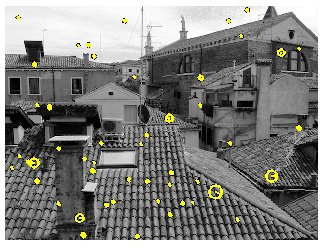
\includegraphics[width=4.5cm, height=4.5cm]{./Pictures/SIFT/siftDescriptorExample.jpg}
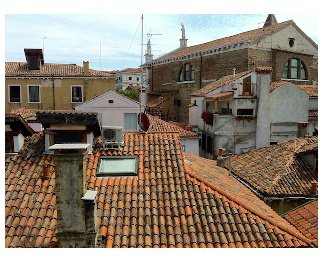
\includegraphics[width=4.5cm, height=4.5cm]{./Pictures/SIFT/siftExample.jpg}
\caption{Example of SIFT Descriptors}
\label{fig:siftExample}
\end{figure}
\end{center}
%%%%%%%%%%%%%%%%
SIFT features are very useful for finding objects or recognizing scenes in an image. SIFT descriptors were first introduced by \citet*{lowe} in ICCV1999. They took the idea from the vision process in primates. The SIFT Features are actually similar to the neurons in inferior temporal cortex of a primate. Features are efficiently extracted through a staged filtering approach that focuses on some key invariable points in scale space. The steps of this filtering approach are mentioned in Figure \ref{fig:siftProcess}.
 %%%%%%%%%%%%%%%
 \begin{center}
\begin{figure}
\centering
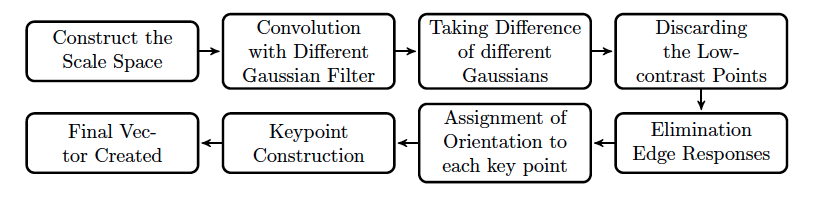
\includegraphics[width=\linewidth]{./Pictures/SIFT/siftSteps.jpg}
\caption{Process Flow of SIFT Descriptor }
\label{fig:siftProcess}
\end{figure}
\end{center}
%%%%%%%%%%%%%%%%
SIFT features have been proven very useful in objectives like natural scene recognition \citet*{naturalSceneRecognition}. These features are also very useful in object recognition, this was shown in \citet*{lowe}. Motivated by the excellent performance of SIFT Features in Image Categorization, we chose SIFT as one of visual features, we were going to use for image classification purpose.

\Citet*{naturalSceneRecognition}  has been shown that dense local scale-variant features performs better compared to sparse features. We. therefore, extracted dense SIFT features of $16 \times 16$ pixels frames. These frames were created over a grid with spacing of 8 pixels. A dense image descriptor has better chance to associate itself to overall scene recognition as it can capture uniformity of image such as landscapes, sea, sky etc. 

We used the VLFEAT Library for finding the SIFT descriptors. Once, we had obtained the SIFT descriptors for the full set of images, we 
constructed a visual vocabulary of 400 visual words as described in \citet*{bagOfWords}. \Citet*{bagOfWords} introduced the 
concept of visual bag of words, because this methodology overcomes the problem of high-dimensionality of SIFT features, quite intelligently. Using these bag of words, we could constraint the definition of a visual concept in these 400 visual words, which also provided efficiency and robustness. We used k-means from VLFEAT library \citet*{vlfeat} for creating 400 clusters from the full training 
data. In figure \ref{fig:siftMatching}, we have given an example of using SIFT Bag of Words features to match two natural scenes. In these images, we can see the SIFT descriptors with green circles. We have also shown the connection (an edge with blue line) matching these SIFT descriptors on both the images. We can see that SIFT descriptors calculated on image 1 also exist in image 2, hence these two images matches.

%{\bf *** How does matching actually happen? It is not clear from your
%figures. Explain in more detail. ***}

%%%%%%%%%%%%%%%
 \begin{center}
\begin{figure}
\centering
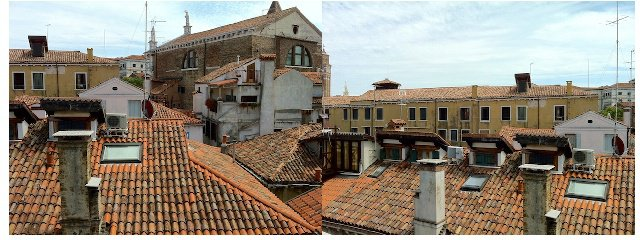
\includegraphics[width=\linewidth]{./Pictures/SIFT/siftMatching.jpg}
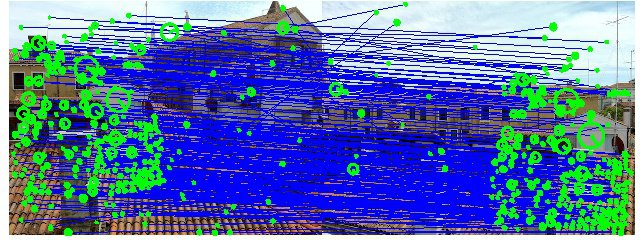
\includegraphics[width=\linewidth]{./Pictures/SIFT/siftMatchingDescriptor.jpg}
\caption{Use of SIFT Descriptor in matching }
\label{fig:siftMatching}
\end{figure}
\end{center}
%%%%%%%%%%%%%%%%
\Citet*{bagOfWords} extended the normal BoW (Bag of Words model) by introducing the Spatial Pyramid technique. In this technique, we create a spatial pyramid of an image by dividing the image in hierarchical spatial layers. Each division provides a finer sub-region and more spatially localized information about the image. 

We keep on dividing the image in layers and then calculate histogram over those 400 Visual words on these divisions.This approach gives improved results on challenging scene recognition tasks as shown by  \citet*{bagOfWords}. 

We also used the Spatial Pyramid technique as defined in \citet*{bagOfWords}. We did 2-level Spatial partitioning. In level 0, we had the full image, this gave a 400 dimensional vector (the size of bag of visual words). In level 1, we partitioned the image in 4 sub regions, This gave $4 \times 400$ dimensional vector. In level 2, we again partitioned each sub-region into 4 sub-regions, so we obtained $4 \times 4 =\  16 $ sub-regions.This gave us a $16 \times 400 $ dimensional descriptor. In this way, we have an image descriptor of size $8400$. We used the MATLAB implementation developed by \citet*{bagOfWords} for computing the pyramid on the SIFT descriptors.

%%%%%%%%%%%%%%%
 \begin{center}
\begin{figure}
\centering
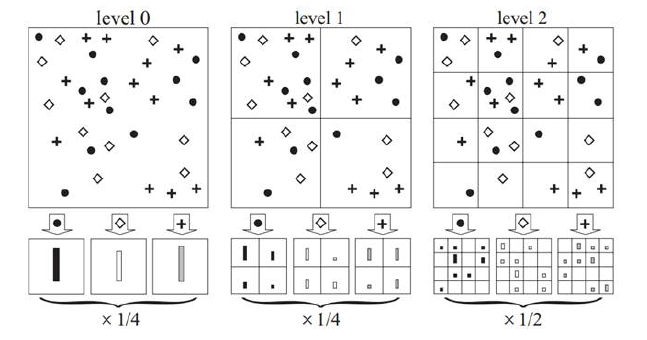
\includegraphics[width=\linewidth]{./Pictures/SIFT/pyramidCompute.jpg}
\caption{Computation of Spatial Pyramid over an image }
\label{fig:pyramidCompute}
\end{figure}
\end{center}
%%%%%%%%%%%%%%%%
A schematic diagram of  calculating Spatial Pyramid of an image is shown in figure \ref{fig:pyramidCompute}. In figure \ref{fig:pyramidCompute}, we have represented the construction of the spatial pyramid. In this case, we have a dictionary of three visual words represented by plus, circle and rhombus. The image is partitioned in 3 layers and for each layer in each sub-division, the count of each visual words is used to create the bin and then the spatial pyramid bins are weighted as given in \citet*{bagOfWords}.
%%%%%%%%%%%%%%%%%%%%%%%%%%%%%%%%%
%%%%%%%%%%%%%%%%%%%%%%%%%%%%%%%%%
\subsection{GIST Features}
Just like SIFT features, GIST features also have their roots in the concept of primate vision. GIST features were first introduced by \citet*{GIST} in 2001. They took the reference of paper \citet*{barrow} which describes vision in humans. 
 
In case of scene recognition, human system actually does progressive reconstruction of the input of local descriptors (edges, surfaces) integrated into complex decision layers. Therefore, the recognition of read word pictures may be initiated from some basic global descriptors, ignoring most of the details and object data.
\Citet*{GIST} suggested that recognition of real world pictures can be attempted with some small set of perceptual dimensions:  \emph{ruggedness, naturalness, roughness, expansion, openness}. This small set of perceptual dimensions can be used as a way of recognizing a picture without going into the tiresome process of segmentation and processing individual regions/objects. This low -dimensional representation is termed as "Spatial Envelope" in \citet*{GIST}. These Spatial Envelope Perceptual Dimension Descriptors can be reliably computed using spectral and coarsely localized information.

The model based on this spatial envelope generates a multidimensional space. In this projected space, scenes with semantically close categories (e.g. sea, water, river, lake) are projected closely. The performance of this model emphasizes that for scene categorization and modeling a holistic representation of a scene, we do not need specific information about object shape or identity. This holistic representation is defined as the GIST of the scene.

\citet*{douze} have shown that the GIST descriptor is very efficient and useful for web-scale search systems for images. This indicates that GIST can also be an efficient feature for image classification. We, therefore, include GIST in our visual feature list.

We used the GIST implementation available at \citet*{gistWebSite} given by \citet*{GIST}. We first decomposed the image using filters of 8 orientations for each of the 4 scales mentioned in \citet*{GIST}. We got 32 oriented filters by this way.Then, the image was represented as a $4 \times 4 $ matrix. Output values of all filters were normalized to $4 \times 4 $ matrix. Then, the image was represented by the weighted combination of all these values giving 8(orientation)$\times$4(scales)$\times$4$\times$4(size of matrix) $=$ 512 dimensional vector.

GIST can be easily handle large databases because it is memory efficient and also computationally efficient. It categorizes natural 
images very well.
 %%%%%%%%%%%%%%%
\begin{center}
\begin{figure}	
\centering
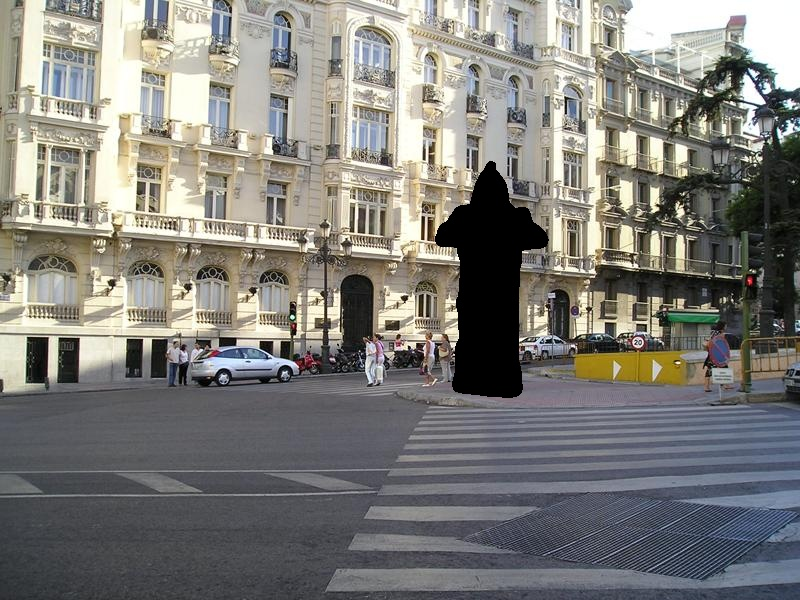
\includegraphics[width=4.5cm, height=4.5cm]{./Pictures/GIST/gistImage.jpg}
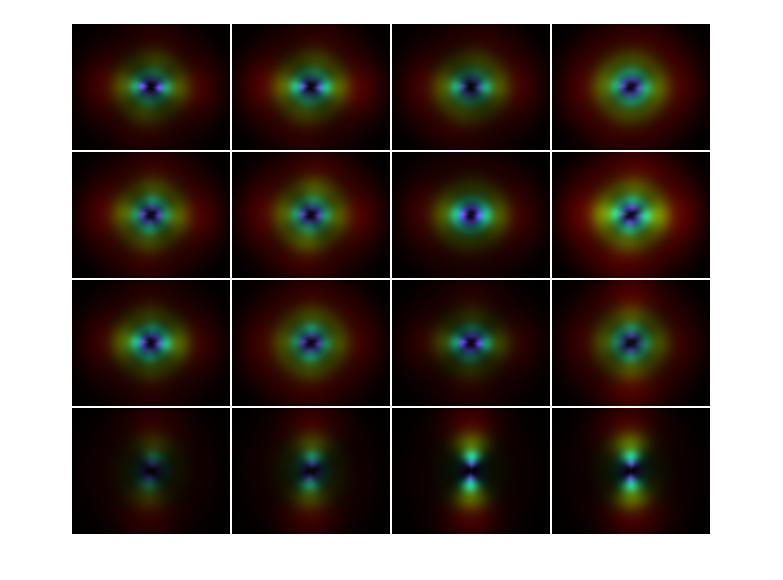
\includegraphics[width=4.5cm, height=4.5cm]{./Pictures/GIST/gistExample.jpg}
\caption{Example of GIST descriptors}
\label{fig:gistExample}
\end{figure}
\end{center}
%%%%%%%%%%%%%%%%  		
In Figure \ref{fig:gistExample}, we have shown GIST descriptors of an image. The left part is an image from our database and on the 
right is the GIST descriptor for the image.
 %%%%%%%%%%%%%%%%%%%%%%%%%%%%%%%%%

 %%%%%%%%%%%%%%%%%%%%%%%%%%%%%%%%%
 %%%%%%%%%%%%%%%%%%%%%%%%%%%%%%%%%
\subsection{COLOR Space Features}
Colors for each pixel in an image can be represented using tuples of numbers, numbers can be three as in RGB model or four as in CMYK 
model. A color space is a way to represent colors, it is also called a color model or color system. Every color can be represented by a point in this color space. There are multiple color spaces, which are used to represent a color according to the application. Some of them are RGB , CMYK , HSV, CIELAB. In this section, we will give a brief overview of RGB and CIELAB, because we used these in our visual features.

\subsubsection*{RGB Color Space}
RGB color space consists of three components Red, Green and Blue. Red, Green and Blue are considered as additive primary colors 
because these colors can be used to create a broad range of colors. 

Colors can be created on computer monitors with color spaces based on the RGB color model, using the additive primary colors (red, green, and blue). In every pixel, we define the color using intensity values for each of these three colors. The range of intensity values is 0-255. This leads to 16,777,216 different colors, when used in different combinations of each of these colors. It is a reproduction medium dependent color space because it depicts different RGB values for the same image when computed on different devices, such as the phosphor (CRT monitor) or backlit (LCD monitor). RGB color space has been used in most modern display devices like Television, Computers, Mobile Phone displays etc.

\subsubsection*{CIELAB Color Space}
CIELAB Color Space describers all colors which are perceptibly visible for human beings. It was first introduced by \citet*{CIELAB},
International Commission on Illumination in 2003. It is also a three dimensional color space with three components. The three components in CIELAB are $L*$,$ a*$ and $b*$. $L*$ represents the lightness of color ranging from 0 to 100 in which 0 is black and 100 is white. 
$a*$ and $b*$ are color spaces. The range of both of these are 128 to +127. In this $a*$(+127) represents red color where as 
$a*$(-128) represents green color. $b*$(+127) represents yellow color where as $b*$(-128) represents blue color. 

To convert an image from CIELAB to RGB, we first converted the RGB image to CIEXYZ color space. Then we converted CIEXYZ to CIELAB. 
For doing this, we used MATLAB functions (makecform, applycform). The formulas for converting RGB color space to CIELAB are as follows:
First conversion is from RGB to XYZ and then we convert this into CIELAB. Conversion formula is mentioned below. 
Conversion from CIEXYZ space to CIELAB space:
		 $$ \left( \begin{array}{c} X \\ Y \\ Z \end{array} \right) =  \left( \begin{array}{ccc} 0.412453 & 0.357580 & 0.180423 \\ 0.212671 & 0.715160 & 0.072169 \\ 0.019334 & 0.119193 & 0.950227 \end{array} \right) \left( \begin{array}{c} R \\ B \\ G \end{array} \right)$$
		 \[
L^{*} =
  \begin{cases} 
      \hfill 116 \times (\frac{Y}{Y_n})^{({\frac{1}{3}})}    \hfill & \text{ if $(\frac{Y}{Y_n}) > 0.008856$ } \\
      \hfill 903.3 \times (\frac{Y}{Y_n}) \hfill & \text{otherwiise} \\
  \end{cases}
\]
 \[  a^* = 500 \times (f(\frac{X}{X_n})-f(\frac{Y}{Y_n})) \\ \]
   \[  b^* = 200 \times (f(\frac{Y}{Y_n})-f(\frac{Z}{Z_n}))\\ \]
 where,
  \[
  f(x)=
   \begin{cases} 
   \hfill x^{\frac{1}{3}} \hfill & \text{ if $( x > 0.008856)$ } \\
   \hfill 7.787 \times t + \frac{16}{116} \hfill & \text{,otherwise.} \\
   \end{cases}
  \]
 Here $X_n$, $Y_n$, and $Z_n$ are the tri-stimulus values of the 
reference white. 

\subsubsection*{Color Histogram}
The Color Histogram is a very prominent talked feature in image classification problems. Color Histogram is a way to represent the cumulative distribution of colors in an image. It calculates the number of pixels that lie in a particular color range. The color ranges are histogram bins for the color histogram model. Color Histograms are independent to rotation of the image. Therefore, even if the image is 
tilted, it won't affect the classification. Apart from this, computational efficiency is another strong reason behind using color histograms in classification problems. The disadvantage of color histogram is that it fails to capture the spatial distribution of the color in images and only captures the color information.

As we described earlier in RGB color space subsection, RGB color space is dependent on the device.  We, therefore, do not choose it for our color histogram because of it being device dependent 

CIELAB color space appears to be a better choice because of its perceptual uniformity and device independence. Perceptual Uniformity means same quantity of perceptual effect is generated with same quantity of change in color values or we can say that visual effect is proportional to color values.

We first used inbuilt MATLAB functions to convert the given images from RGB space to CIELAB color space. After that we calculated the color histogram after dividing the image into 16 parts called blocks. Now we constructed bins of 4 for each L,  a and b component. Thus we had a total of 64 color bins. Thus for each block we get a 64 dimensional color histogram. When we combine the vectors we get a 
vector of $(16 \times 64 ) =1024$ dimensionality.
   
\subsection{Texture/ GLCM Feature Extraction}
In order to extract some meaningful information from an image, it is important to get some human interpretable features from the image. There are three types of such features which lead to perceptive interpretation of color images: spectral, textual and contextual features.

In such human interpretable features, texture is an important feature. In normal terms, we can define texture of an image in estimate of smoothness of that image. In everyday terms, texture can be defined with words as rough, bumpy or silky.

A texture, which is rough, when touched has large difference between high and low points and the distance between those points is very 
low. A smooth texture will usually have small difference between high and low points with these points being distant.

Image texture also works in the same way. Except the high and low values, we have brightness values (also referred as grey levels), instead of elevation. Instead of using hand or finger to judge the surface, a window or box is used to define the size of probe.

GLCM or Gray Level Co-occurrence Matrix acts like a texture indicator for an image. This co-occurrence matrix represents the inter-pixel distance and spatial relationship between gray values over an image. This spatial interrelation of the grey tones actually determines the textural pattern. It was first introduced by \citet*{haralick}, so these are also called Haralick features . 

For calculating GLCM features for an image, we first converted it to a gray-scale image, because GLCM is actually an estimate of 
the occurrence of different combinations of pixels in a gray-scale image. 

The gray level co-occurrence matrix $G(i,j,\theta, d)$ can be calculated as follows. The value of $G(i,j,\theta, d)$ is count of occurrences of the pair of pixels having gray value $i$ and $j$, where the distance between these pixels is $d$ and direction specified by angle $\theta$. In standard GLCM matrix, the angles used are 0\textdegree, 45\textdegree, 90\textdegree and 135\textdegree with 
$d=1\ pixel$. This directional component of $\theta$ makes it more powerful in the sense that it represents features from every angle of 
an image.
  %%%%%%%%%%%%%%%
 \begin{center}
\begin{figure}
\centering
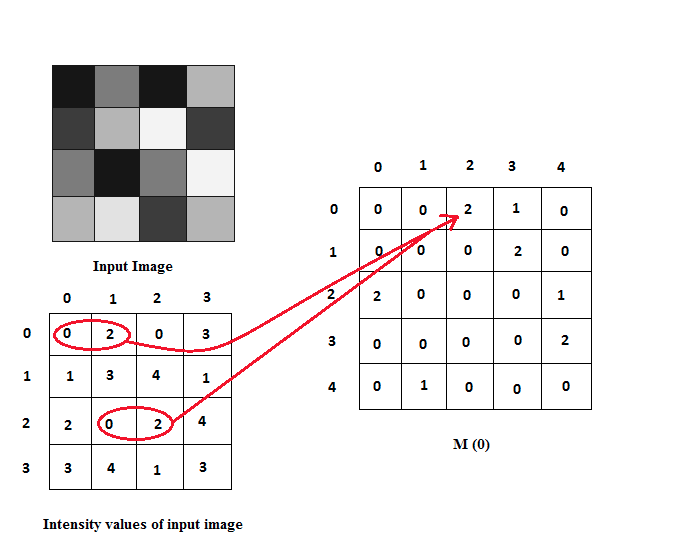
\includegraphics[width=\linewidth]{./Pictures/GLCM/process.jpg}
\caption{Co-occurence Matrix G(0\textdegree) generation for N=5 levels }
\label{fig:glcmMatrix}
\end{figure}
\end{center}
%%%%%%%%%%%%%%%%
Figure \ref{fig:glcmMatrix} illustrate the process of finding co-occurrence matrices using $N=5$ levels. It is showing gray-scale co-occurrence G(0\textdegree,$d=1$). We can observe that pixels (0,2) of the input is shown in G(0\textdegree,$d=1$) as 2 because we only have two occurrences of the pixel intensity value 0 with horizontally adjacent pixels with intensity = 2 in the input. We computed the matrix  
G as symmetric, as we considered pair (0, 2) as (2, 0) as well. Matrix G can also be computed with non-symmetric measure.

In our approach, we computed $G$ for all $\theta$ angles using $N=8$ with symmetry because increasing the gray levels further was decreasing the accuracy and lesser number of gray levels might not be sufficient to capture the texture adequately. We used MATLAB 
functions to get this matrix. This step gave us four $8 \times 8$ matrices. As input is not re-sized to some predefined dimensions, we 
normalized each matrix for better comparison. After normalization, 
we got a $1\times 64 $ dimensional vector for each matrix. We merged 
these to get $1\times 256 $ size vector for an image.

\subsection{HOG-LBP Features}
HOG or Histogram of Oriented Gradients is a widely used 
feature for object recognition in Computer Vision. The idea behind 
this descriptor is that the object in an image can be characterized by the 
intensity gradients or distributed edge directions. HOG 
descriptor works in a localized region, therefore it does not get 
affected with illumination changes or geometric transformations like 
rotation, scale, or change in viewpoint. These descriptors were 
first used by \citet*{HOG} for pedestrian detection in 2005. After that these descriptors clubbed with LBP features are usually 
used for object recognition \citet*{hog1}, \citet*{hog2},\citet*{hog3} etc. 

The steps for constructing HoG descriptors are shown in figure \ref{fig:hogProcess}.
%%%%%%%%%%%%%%%
 \begin{center}
\begin{figure}
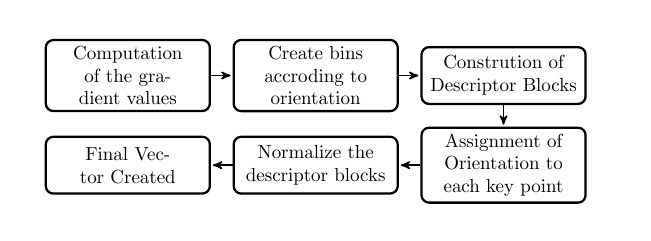
\includegraphics[width=\linewidth]{./Pictures/HOG/hogProcess.jpg}
\caption{Construction of HoG descriptors }
\label{fig:hogProcess}
\end{figure}
\end{center}
%%%%%%%%%%%%%%%%
Local Binary Pattern (LBP) is a texture classification feature. It was first 
introduced by  \citet*{ojala} in 1994. LBP captures the 
appearance of an image in a neighborhood of the pixel. A LBP is a 
string of bits, which contains one bit for each of the pixels in
the neighborhood. LBP does not get affected by monotonic gray level 
changes and acts as a good discriminator. 

\citet*{WangHOG} tried combining HoG with LBP. The results indicated 
high improvement in performance in case of object detection. If the image is cluttered with 
blurred edges,  HoG loses its discriminating capability,  LBP acts as a complementary feature to HoG in such 
cases. LBP uses uniform patterns to remove the noisy edges from a 
cluttered image. \citet*{santana} have shown 
that the combination of HoG and LBP acts much better than each 
individually. We, therefore, considered a combination of HoG and LBP 
for our classification. 

We used VLFEAT \citet*{vlfeat} library for computing HoG features. 
VLFEAT has two variants of HoG. One is UoCTTI variant, other is 
Dalal and Triggs's variant (\citet*{HOG}). We computed the UoCTTI 
variant HoG on each painting. This variant computes directed and 
also undirected gradients. Apart from this, it also has 4-
dimensional texture-energy feature on a window size of $16 \time 16$. 
We therefore obtained 31 dimensional HoG vector for each cell.

For computing LBP features, we again used VLFEAT library (\citet*{vlfeat}).  
VLFEAT considered a $3*3$ neighborhood, this lead to LBP features that is 
a 8 bit long string vector. This 8 bit long vector can assume $2^8 = 256$ 
possible values. These 256 possible values were further quantized into a smaller number of patterns. This uniform quantization makes LBP features computationally efficient.

In this uniform quantization, we made the following observations. There 
was one quantized pattern, for every bit, which has exactly one 
transition from 0 to 1 and one from 1 to 0 when scanned in 
anti-clockwise order. Plus one pattern comprised of two uniform 
LBPs and one pattern comprised all other LBPs. These observations 
yield a total 58 patterns. When we concatenated both HoG and LBP 
vector descriptors we get combined vector of 89 dimensions. We further used
the bag of words approach on this combined HoG-LBP vector. We formed a bag(visual dictionary)
of 4000 visual words using K-means implementation of VLFEAT and after that we combined the 
histogram on this visual dictionary for each vector, which gave a 
vector of 4000 dimension for each image.
%{\bf *** What is k-means doing here? It is not clear. ***}
% I meant K-means implementation of VLFEAT for finding some visual words over which we can combine the histograms.
%%%%%%%%%%%%%%%%
 \begin{center}
\begin{figure}
\centering
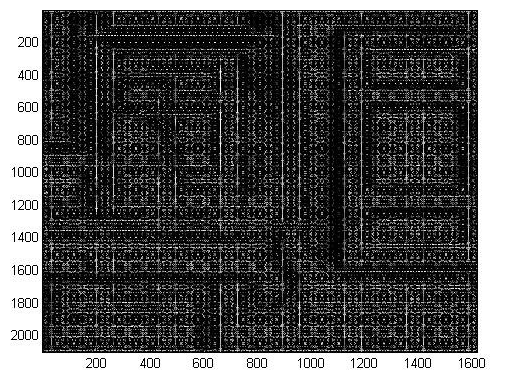
\includegraphics[width=4.5cm, height=4.5cm]{./Pictures/HOG/hogFeatures.jpg}
\caption{Example of HOG Descriptors}
\label{fig:hogExample}
\end{figure}
\end{center}
%%%%%%%%%%%%%%%%%
In figure \ref{fig:hogExample}, we have  shown the HOG descriptor on 
an image. The left part is the original image and the right part shows 
the HoG descriptor for the image.

\section{Social Content Based Feature Extraction}
Social meta-data obtained from images had similar properties like a text data-set, because we had tags, comments, groups all in normal 
language text. So, It makes sense to just use text processing methods here. But, this text data also had inherited 
structure of a social network. We, therefore, tried to utilize this extra 
aspect, first constructed node features over the social-metadata for 
each image as shown by \citet*{Jure}. These node/social feature 
vectors had high dimensionality. We, therefore, used the topic 
modeling/text processing methods over these social features to 
construct a better and reduced representation. \Citet*{tang} have shown that such topic-level modeling of social-
networking data leads to good results in finding patterns and making 
inferences. These final low-dimensional features projected the 
semantically close node features (like mountain, hill etc.) near to 
each other. We tried Latent Semantic Indexing(LSI), Latent Dirichlet 
allocation (LDA) and Random Projection (RP) methods for the purpose 
of dimesionality reduction and topic modeling. 
The process of constructing useful feature vectors from the social 
meta-data obtained can be divided into the following steps:
\begin{itemize}
\item Pre-analysis of Social Data
\item Constructing Node Features
\item Applying Topic Modeling/Text Processing Methods on Binary Social Features
\end{itemize} 
In what folows we will discuss each of these steps.
\subsection{Pre-analysis of Social Data}
Preliminary  observations of the data suggest that 
tags are less structured, are provided by any number of annotators 
and can include the information that is not easily detectable from 
content alone, such as location for example sea-side or mountain ranges. 
Groups are similar to tags, with the difference that the groups in which 
an image is featured, are chosen entirely by the image's author.

\subsection{Constructing Node Features}
There are some properties, which can be defined for a single image 
instance, e.g. tags, groups etc. We call such features as node 
features, because these properties can be separately defined for 
each image/node. 

We first constructed an indicator vector via encoding those words, groups and 
tags that appear in an image. For this, we first consider the 1000 
most popular words, groups and tags across the entire data-set . As 
described in \Citet*{Jure}, this data set of only 1000 most popular 
words did not sufficiently represent the whole data. We, therefore, 
also considered any words, groups and tags that are at least twice as 
frequent in images having the label in question compared to the 
overall rate. This way we got similar node features as described in \citet*{Jure}. 

For developing this word feature, we utilized text from the image's 
title, it's comment thread and description after eliminating stop-words.
This will give us more than 40000+ points. The node-feature vector 
was in binary form and had high dimensionality. We had 0 and 1 as the 
value for each field in this vector corresponding to the presence of the 
word in the image data or not. We further converted this raw binary 0 
and 1 form, to usable social features with the use of text 
processing methods like Latent Semantic Indexing and Random 
Projections.

\subsection{Applying Text Processing/Topic Modeling Methods on 
Binary Social Features}
We, now, use dimensionality reduction cum text processing methods 
on these feature vectors. For text processing, we can consider 
each image as a document and the current node feature vector as a 
representation of the dictionary. This vector represents the presence of 
a word in the document. Now, we have a corpora of word features and in 
the next step, we just need to use some topic modeling/text processing 
methods to get a feature vector with reduced dimension.

We experimented with Latent Semantic Indexing, Random Projection and 
Latent Dirich-let Allocation as some possible methods to do such 
dimensionality reduction for sparse binary data.
\subsubsection{Latent Semantic Indexing}
Latent Semantic Indexing is actually a singular value decomposition 
method to identify patterns in the relationship among the semantic 
concepts in an unstructured collection of text. It is normally used 
for extraction of conceptual content of a body of text by 
establishing associations between those words which show a 
similar contextual presence.In \citet*{Deerwester}, 
LSI is used in a variety of information retrieval and text 
processing applications which are increasingly used for electronic 
document discovery, publishing, government/intelligence community. 
\citet*{e-discovery}.

In typical information retrieval methods information is retrieved 
by literally matching terms in in the search space with those of the 
search query. However, this method, which depends purely on lexical 
matching, can be inaccurate. Since, there are many ways to express a given 
concept literal matching may not provide us the 
relevant information. A better approach will be to create a basis for 
conceptual topic in the search space. Latent Semantic Indexing 
tries to overcome the problems of lexical matching by using 
statistically derived conceptual indices instead of raw data. Latent 
Semantic Indexing  assumes that there is a hidden latent conceptual 
structure in raw features which is not visible because of 
variability of word choices. A truncated SVD (Singular Value 
Decomposition ) is used to estimate this latent semantic structure. 
These statistically derived vectors prove to be more robust 
indicators of information than individual terms. 

\subsubsection*{Basic Concept}
Latent Semantic Indexing is a technique that projects the feature 
vectors into a space with "latent" semantic dimensions. In latent 
semantic space,  two feature vectors can have high cosine similarity 
even if they do not share any terms - as long as their terms are 
semantically similar in a sense to be described later. We can look 
at LSI as a similarity metric that is an alternative to word overlap 
measures like tf.idf. 
In terms of topic modeling and text processing, latent semantic 
indexing is the application of Singular Value Decomposition or SVD, 
to a "word-by-document" matrix. The projection into the latent 
semantic space is chosen such that the representations in the 
original space are changed as little as possible when measured by 
the sum of the squares of the differences. 

SVD represents a matrix $A$ as $\hat{A}$ in a lower dimensional 
space such that the "distance" between the two matrices (Which is 
measured by the 2-norm is minimized): 
\footnote{ The 2-norm for matrices is the equivalent of Euclidean distance for vectors.}
		$$ \delta = \| A - \hat{A} \| _{2}$$
SVD projects an n-dimensional space onto a k-dimensional space where 
$n \ll k$. Thus, the projection transforms a feature vector in 
n-dimensional word space into a vector in the k-dimensional reduced 
space. 
We used the GENSIM library (\citet*{gensim}) in Python for Latent Semantic 
Indexing of our data. It was developed by \citet*{radimrehurek} for topic modeling with large corpora.
		 
\subsubsection{Latent Dirichlet allocation}
Latent Dirichlet allocation (LDA) is another frequently used 
process in natural language processing. It is a generative model 
that allows a set of observations to be depicted by unobserved groups 
explaining why some parts of the data are quite similar. For example 
in a general natural language processing scenario, when the 
observations are words associated with a document, it 
assumes a document is a mixture of a small number of topics and that 
each word's presence is dedicated to one of the document's concepts. 
LDA was actually a graphical model presented in \citet*{Blei} for 
topic discovery.  LDA has connection with image classification 
because in \citet*{Li} a variation on LDA was used to automatically 
split the natural images into categories, such as  forest and 
mountain, by assuming the images as words. 
Latent Dirichlet allocation uses a generative probabilistic 
model of a corpus. The basic idea is that documents are represented 
as random mixtures over latent topics, where each topic is 
characterized by a distribution over words. There are many variants 
of LDA. In \citet*{Blei}, LDA assumes the following generative process 
for each document $w$ in a corpus $D$:
	\begin{itemize}
	\item Choose $N \sim Poisson(\xi)$.
	\item Choose $\theta \sim Dir(\alpha)$.
	\item For each of the N words wn:
	\begin{itemize}
		\item  Choose a topic $z_n \sim Multinomial(\theta).$
		\item Choose a word $w_n$ from $p(w_n | z_n,\beta)$, a multi nomial probability conditioned on the topic $z_n$.
	\end{itemize}
	\end{itemize}
%%%%%%%%%%%%%%%%%
 \begin{center}
\begin{figure}
\centering
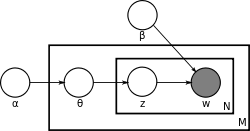
\includegraphics[width=\linewidth]{./Pictures/Latent_Dirichlet_allocation.png}
\caption{Plate Model for  LDA  \citet*{Blei}}
\label{fig:ldaExample}
\end{figure}
\end{center}
%%%%%%%%%%%%%%%%
In figure \ref{fig:ldaExample}, we have shown plate model of Linear 
Discriminant Analysis. With plate notation, the dependencies among the many variables can be captured concisely. The boxes are plates representing replicates. The outer plate represents the documents, while the inner plate represents the repeated choice of topics and words within a documents. M denotes the number of documents. N the number of words in a document. $\alpha$ is the parameter of the Dircihlet prior on the per-document topic distributions, $\beta$ is the parameter of the dirichlet prior on the per-topic: word distribution, $\theta_i$ is the topic distribution for document i, $\phi_k$ is the is the word distribution for topic k,$z_{ij}$ is the topic for the jth word in document $i$, and $w_{ij}$ is the specific word.The $w_{ij}$ are the only observable variables, We can then mathematically describe the random variables as follows:

\begin{itemize}
\item $\phi_{k=1.......K} \sim Dirichlet_V(\beta)$\\
\item $theta_{d=1 \dots M} \sim Dirichlet_K(\alpha)$ \\
\item $z_{d=1.......M,w=1....... N_d} \sim Categorical_K(\theta_d)$ \\
\item $w_{d=1 ....... M,w=1....... N_d} \sim Categorical_V(\phi_{z_{dw}})$ \\
\end{itemize}


%{\bf *** You seem to be confusing Latent Dirichlet Allocation with the
%other LDA - Linear Discriminant Analysis. Which LDA are you talking
 %about? The figure is for Linear Discriminant Analysis and not
%Latent Dirichlet Allocation. ***}
%Yes sir, this was  a mistake.
In our case the LDA did not provide good results because we 
already have textual data which is oriented to solve a binary 
classification problem. This binary nature of a topic leads to too 
sparse feature generation from Latent Dirichlet allocation (LDA). 
This sparseness of features around images lead to low quality 
classification. LDA also fails if discriminatory information is
not in the mean but in the variance of the data  \citet*{Blei}. We, 
therefore, discard this method for our computations.

\subsubsection{Random Projections}
Random Projections is a powerful methods for dimensionality 
reductions in image and text data (\citet*{randproj}).  
In \citet*{rpCite}, Bingham introduced random projections as a 
simpler and less erroneous dimensionality reduction tool for 
information retrieval from text and processing of images. It is 
very useful in cases where reduction of high 
dimensional data to low dimensions is essential. Which if not done
leads to heavy computation penalty without significant gain. 
Using random projection is significantly less expensive compared to 
techniques like principal component analysis. In random projection, 
the original high dimensional data is projected onto a lower 
dimensional subspace using a random matrix $R$. 
In random projection, the original d-dimensional data is projected 
to a k-dimensional $(k << d)$ subspace through the origin, using a 
random $k \times d$ matrix $R$ whose columns have unit lengths. 
Using matrix notation where $X_{d\times N} $ is the original set of 
N d-dimensional observations,
$$ X^{RP}_{k\times N} = R_{k\times d} X_{d\times N} $$
is the projection of the data onto a lower k-dimensional subspace. 
The key idea of random mapping arises from the Johnson-Lindenstrauss 
lemma \citep{lemma}: if points in a vector space are projected onto a 
randomly selected subspace of suitably high dimension, then the 
distances between the points are approximately preserved.   
We write the Euclidean distance between two data vectors $x_1$ and 
$x_2$ in the original large-dimensional space as 
$\lVert x_1 - x_2 \rVert$. After the random projection, this 
distance is approximated by the scaled Euclidean distance of these 
vectors in the reduced space:
$$\sqrt{ d/k} \norm{R_{x_1} - R_{x_2}}$$
where d is the original and k the reduced dimensionality of the data 
set. The scaling term $\sqrt{d/k}$ takes into account the decrease 
in the dimensionality of the data: according to the 
Johnson-Lindenstrauss lemma \citep{lemma} the expected norm of a projection 
of a unit vector onto a random subspace through the origin is $\sqrt{k/d}$
The choice of the random matrix R is one of the key points of 
interest. The elements $r_{ij}$ of R are often Gaussian distributed,
but the Gaussian distribution can be replaced by a much simpler 
distribution such as
\[
	r_{ij} = \sqrt{3}*\begin{cases} 
	 +1 & \textrm{with proabibility $\frac{1}{6}$} \\
	 0 & \textrm{with proabibility $\frac{2}{3}$}\\
	-1 & \textrm{with proabibility $\frac{1}{6}$} \\
		\end{cases}
\]
In fact, practically all zero mean, unit variance distributions of 
$r_ij$ would give a mapping that still satisfies the Johnson-Lindenstrauss
lemma. This means further computational savings in feature 
computation, as the computations can be performed using integer 
arithmetic. Again for computing the random projections, we used the 
GENSIM library \citep{gensim} in Python.  
It has been found that even though it is computationally light, 
Random projections is a sufficiently accurate method for 
dimensionality reduction of high dimensional data \citet*{Dasgupta}.

\subsection{Implementation of Dimensionality reduction}

Considering that we are using a large database and we need to do 
dimensionality reduction for such data. We use an online version 
of aforementioned techniques. So that we don't have to bother about 
loading the whole data into memory. 

Both LSI and RP rely on TF-IDF (term frequency - inverse document 
frequency) as a fast pre-processing step.  
\citet*{radimrehurek} gives a framework \citet*{gensim} for doing all 
this text processing on large corpora in memory independent fashion. 
We use this as a tool for doing LSI and RP Computation. On varying the 
number of dimensions in dimensionality reduction we found that 
using 300 features in LSI and 400 features in RP gives us the best 
results.

In selecting the dimension the whole point is to reduce 
dimensionality in such a way that we can use kernel methods which would 
be too costly and too susceptible to over-fitting with thousands of 
binary features.
We directly converted the node features of dimension 40000+ in social 
features to dimension 300 (LSI) and dimension 400 (RP).  This 
conversion was done in Python using GENSIM and the converted 
files are in the LIBSVM format. 

